\documentclass{beamer}
%
% Choose how your presentation looks.
%
% For more themes, color themes and font themes, see:
% http://deic.uab.es/~iblanes/beamer_gallery/index_by_theme.html
%
\mode<presentation>
{
  \usetheme{default}      % or try Darmstadt, Madrid, Warsaw, ...
  \usecolortheme{default} % or try albatross, beaver, crane, ...
  \usefonttheme{default}  % or try serif, structurebold, ...
  \setbeamertemplate{navigation symbols}{}
  \setbeamertemplate{caption}[numbered]
}

\usepackage[english]{babel}
\usepackage[utf8]{inputenc}
\usepackage[T1]{fontenc}
\usepackage{algorithm}
\usepackage{algorithmic}
\usepackage{subfig}
\usepackage{stackengine}


% Slide numbers
\addtobeamertemplate{navigation symbols}{}{
    \usebeamerfont{footline}
    \usebeamercolor[fg]{footline}
    \hspace{1em}
    \insertframenumber/\inserttotalframenumber
}

\setbeamertemplate{bibliography item}{\insertbiblabel}

\title[]{Transferring Adversarial Robustness Through Robust Representation Matching}
\author{Pratik Vaishnavi, Kevin Eykholt, Amir Rahmati}
\date{August 2022}

\begin{document}

\begin{frame}
  \titlepage
\end{frame}

% Uncomment these lines for an automatically generated outline.
%\begin{frame}{Outline}
%  \tableofcontents
%\end{frame}

%%%%%%%%%%%%%%%%%%%%%%%%%%%%%%%%%%%%%%%%%%%%%%%%%%

\begin{frame}{Intro}

\begin{itemize}
	\item ML models can be fooled by adversarial examples
	\item Need ways to make models robust to such adversarial attacks
	\item Existing methods are not practical for real-world use
	\item This work proposes a method to transfer robustness
\end{itemize}

\end{frame}

%%%%%%%%%%%%%%%%%%%%%%%%%%%%%%%%%%%%%%%%%%%%%%%%%%
%%%%%%%%%%%%%%%%%%%%%%%%%%%%%%%%%%%%%%%%%%%%%%%%%%

\begin{frame}{}
	
	\begin{figure}
		\centering
		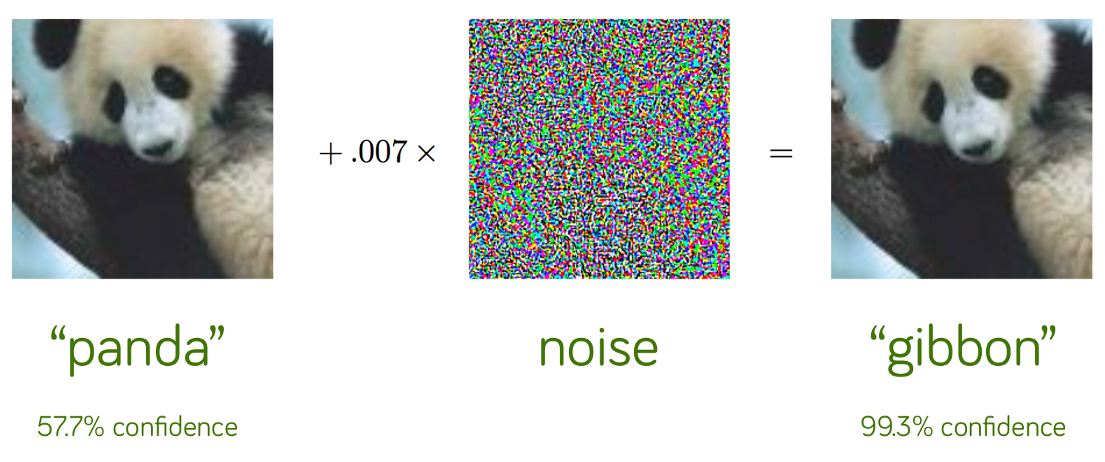
\includegraphics[scale=.25]{./images/adversarial_evasion_attack.png}
		\caption{ML algorithms and especially DNNs are often brittle.}
	\end{figure}
	
\end{frame}

%%%%%%%%%%%%%%%%%%%%%%%%%%%%%%%%%%%%%%%%%%%%%%%%%%
%%%%%%%%%%%%%%%%%%%%%%%%%%%%%%%%%%%%%%%%%%%%%%%%%%

\begin{frame}{Standard Training}
	
	\begin{itemize}
		\item Empirical Risk Minimization (ERM) updates the parameters, $\theta$, of a ANN, $F_\theta$, to minimize the learning model's loss, $L$
	\end{itemize}

	$$\min_{\theta} L(F_\theta(x), y)$$
	
\end{frame}

%%%%%%%%%%%%%%%%%%%%%%%%%%%%%%%%%%%%%%%%%%%%%%%%%%
%%%%%%%%%%%%%%%%%%%%%%%%%%%%%%%%%%%%%%%%%%%%%%%%%%

\begin{frame}{Adversarial Attacks}
	
	\begin{itemize}
		\item Adversarial Evasion Attacks (AEA) attempt to imperceptibly perturb inputs to cause misclassification
		\item Adversaries objective is to add a small perturbation, $\delta < \epsilon$, that maximizes the model's loss
	\end{itemize}

	$$\max_{\delta} L(F_\theta(x+\delta), y)$$
	
	% perturbation, delta, is bounded by some imperceptibility condition, which limits the difference between perturbed and non-perturbed examples
	
\end{frame}

%%%%%%%%%%%%%%%%%%%%%%%%%%%%%%%%%%%%%%%%%%%%%%%%%%
%%%%%%%%%%%%%%%%%%%%%%%%%%%%%%%%%%%%%%%%%%%%%%%%%%

\begin{frame}{}
	
	\begin{figure}
		\centering
		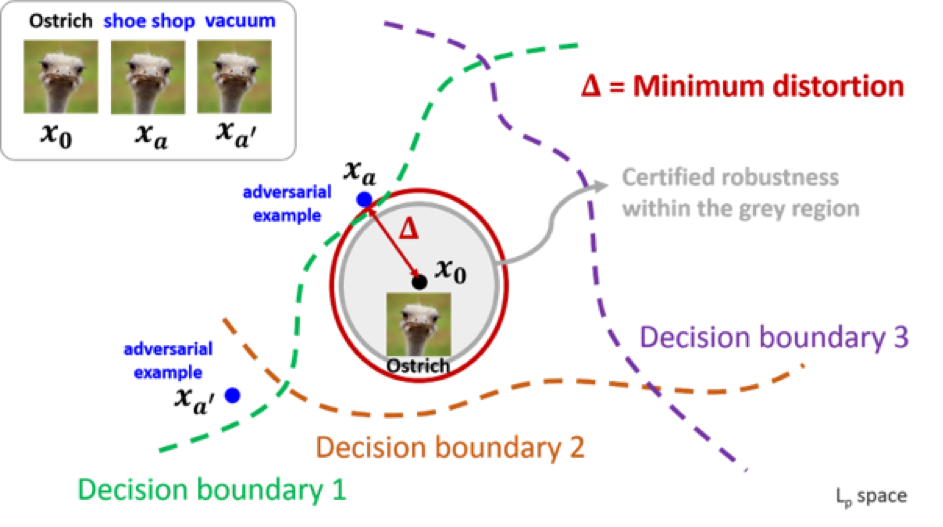
\includegraphics[scale=.7]{./images/adversarial_attack.png}
		\caption{AEAs minimally perturb inputs to attain incorrect classification.}
	\end{figure}
	
\end{frame}

%%%%%%%%%%%%%%%%%%%%%%%%%%%%%%%%%%%%%%%%%%%%%%%%%%
%%%%%%%%%%%%%%%%%%%%%%%%%%%%%%%%%%%%%%%%%%%%%%%%%%

\begin{frame}{Adversarial Defense}
	
	\begin{itemize}
		\item Adversarial Training (AT) \cite{madry2017towards} is the most natural defense 
		\item Attempts to find parameters that minimize the adversary's expected attempts to increase loss
	\end{itemize}

	$$\min_{\theta} \max_{\delta} L(F_\theta(x+\delta), y)$$
	
	% Inner maximization is the attacker's objective
	% Outer minimization makes it harder for attacker to achieve objective

	\begin{itemize}
		% Minimizes the risk over the entire perturbation space, not just the original examples
		\item Essentially, augments the training data with adversarial inputs
	\end{itemize}
	
\end{frame}

%%%%%%%%%%%%%%%%%%%%%%%%%%%%%%%%%%%%%%%%%%%%%%%%%%
%%%%%%%%%%%%%%%%%%%%%%%%%%%%%%%%%%%%%%%%%%%%%%%%%%

\begin{frame}{Adversarial Training}
	
	\begin{itemize}
		\item Several forward-backward passes each iteration vs single pass
		\item Slows training down by order of magnitude
		\item Requires knowledge of attacker's perturbation space
		% Essentially, is not practical for real world use, where models are frequently tweaked, re-trained, compared, re-trained, etc.
	\end{itemize}
	
\end{frame}

%%%%%%%%%%%%%%%%%%%%%%%%%%%%%%%%%%%%%%%%%%%%%%%%%%
%%%%%%%%%%%%%%%%%%%%%%%%%%%%%%%%%%%%%%%%%%%%%%%%%%

\begin{frame}{Explaining Robustness}
	
	\begin{itemize}
		\item Adversarial examples are effective because of a model's tendency to learn non-robust features \cite{ilyas2019adversarial}
		\item Robust models must learn to focus on robust features that are strongly correlated with the input label
		\item Knowledge of robust features could be transferred between models
	\end{itemize}
	
\end{frame}

%%%%%%%%%%%%%%%%%%%%%%%%%%%%%%%%%%%%%%%%%%%%%%%%%%
%%%%%%%%%%%%%%%%%%%%%%%%%%%%%%%%%%%%%%%%%%%%%%%%%%

\begin{frame}{Transferring Adversarial Robustness}
	
	\begin{itemize}
	\item Model robustification should not:
	\begin{enumerate}
		\item reduce performance on non-adversarial examples
		\item be cost prohibitive
	\end{enumerate}
	\item Transferring robustness can eliminate the need to perform AT during retraining and make robustification cost efficient
	% Previous techniques exhibited success only in small perturbation spaces, ie, low generous imperceptibilty condition
\end{itemize}
	
\end{frame}

%%%%%%%%%%%%%%%%%%%%%%%%%%%%%%%%%%%%%%%%%%%%%%%%%%
%%%%%%%%%%%%%%%%%%%%%%%%%%%%%%%%%%%%%%%%%%%%%%%%%%

\begin{frame}{Robust Representation Matching}
	
	\begin{itemize}
		\item Robust Representation Matching (RRM) uses a student-teacher framework to transfer the knowledge of feature importance between models
		\item Trains a teacher model with AT
		\item Trains a student model with combined objective:
		\begin{enumerate}
			\item Minimize the cross-entropy loss, $L_C$
			\item Minimize the robust representation loss, $L_R$
		\end{enumerate}
	\end{itemize}
	
\end{frame}

%%%%%%%%%%%%%%%%%%%%%%%%%%%%%%%%%%%%%%%%%%%%%%%%%%
%%%%%%%%%%%%%%%%%%%%%%%%%%%%%%%%%%%%%%%%%%%%%%%%%%

\begin{frame}{Robust Representation Matching (cont)}
	
	\begin{itemize}
		\item Formally, the training objective for determining the parameters, $\theta$, of the student NN $S_\theta$ is
	\end{itemize}

	$$\min_\theta \biggr [ \lambda \cdot L_C(S_\theta(x), y) + L_R(x) \biggr ]$$
	
	\begin{itemize}
		\item where the robust representation loss is the distance, e.g., cosine similarity, between output of the penultimate layers of the student and teacher models
	\end{itemize}

	$$L_R(x) = d(g_S(x), g_T(x))$$
	
		\begin{itemize}
			\item and $\lambda$ weighs the contribution of the two different objectives
			%\item Higher $\lambda$ weighs standard accuracy more than adversarial accuracy and vice versa
		\end{itemize}
	
\end{frame}

%%%%%%%%%%%%%%%%%%%%%%%%%%%%%%%%%%%%%%%%%%%%%%%%%%
%%%%%%%%%%%%%%%%%%%%%%%%%%%%%%%%%%%%%%%%%%%%%%%%%%

\begin{frame}{Why Match the Penultimate Layer?}
	
	\begin{itemize}
		\item Including the robust representation loss term $L_R$ forces the student to match the teacher's penultimate layer
		\item Matching the penultimate layer can transfer more knowledge than matching the output layer and is architecture-agnostic
		\item Intuitively, these hidden layer's encapsulate the network's understanding of the input and TLDR it seems to work
		\item Previous works used similar strategies \cite{ilyas2019adversarial, goldblum2020adversarially}
	\end{itemize}
	
\end{frame}

%%%%%%%%%%%%%%%%%%%%%%%%%%%%%%%%%%%%%%%%%%%%%%%%%%
%%%%%%%%%%%%%%%%%%%%%%%%%%%%%%%%%%%%%%%%%%%%%%%%%%

\begin{frame}{Adversarial Training Speedup}
	
	% Experiments conducted on CIFAR-10 image classification dataset
	% I truncated their original results to showcase what is most important
		% SAT = standard AT
		% Fast AT = speed up technique applied to SAT
		% Free AT = alternative AT training method
		% RRM = Fast AT applied to RRM
	
	\begin{itemize}
		\item When compared against other AT methods:
		\begin{itemize}
			\item RRM achieves comparable performance to SAT/Fast AT in significantly less training time
			\item RRM achieves greater performance to Free AT in almost the same training time
		\end{itemize}
		\item Attacks conducted using AutoPGD \cite{croce2020reliable}, an iterative form of the FGSM attack \cite{goodfellow2014explaining}
	\end{itemize}
	
	\begin{center}
		\begin{tabular}{ |c|c|c|c| } 
			\hline
			Method & Training Time & Natural Accuracy & Adversarial Accuracy \\
			\hline
			SAT & 1808 & 86\% & 48\% \\
			Fast AT & 193 & 84\% & 50\% \\
			Free AT & 29 & 71\% & 42\% \\
			RRM & 30 & 76\% & 49\% \\
			\hline
		\end{tabular}
	\end{center}
	
\end{frame}

%%%%%%%%%%%%%%%%%%%%%%%%%%%%%%%%%%%%%%%%%%%%%%%%%%
%%%%%%%%%%%%%%%%%%%%%%%%%%%%%%%%%%%%%%%%%%%%%%%%%%

\begin{frame}{Adversarial Robustness Transfer}
	
	% RDT = Robust Data Training
	% KD = Kowledge Distillation
	% Neither works very well in a large perturbation space, eg, a sophisticated attacker
	
	\begin{itemize}
		\item When compared against other transfer methods, RRM vastly outperforms its competitors
	\end{itemize}

	\begin{center}
		\begin{tabular}{ |c|c|c|c| } 
			\hline
			Method & Natural Accuracy & Adversarial Accuracy \\
			\hline
			RDT & 80\% & 1\% \\
			KD & 83\% & 3\% \\
			RRM & 81\% & 46\% \\
			\hline
		\end{tabular}
	\end{center}
	
\end{frame}

%%%%%%%%%%%%%%%%%%%%%%%%%%%%%%%%%%%%%%%%%%%%%%%%%%
%%%%%%%%%%%%%%%%%%%%%%%%%%%%%%%%%%%%%%%%%%%%%%%%%%

% There are is an entire subsection of experiments using a larger dimensional dataset, ResNet
% Essentially demonstrates the same trends
% RRM generalizes welll to high dimensional data

%%%%%%%%%%%%%%%%%%%%%%%%%%%%%%%%%%%%%%%%%%%%%%%%%%
%%%%%%%%%%%%%%%%%%%%%%%%%%%%%%%%%%%%%%%%%%%%%%%%%%

\begin{frame}{Tuning $\lambda$}
	
	\begin{itemize}
		\item Recall RRM's optimization objective:
	\end{itemize}

	$$\min_\theta \biggr [ \lambda \cdot L_C(S_\theta(x), y) + L_R(x) \biggr ]$$
	
	\begin{itemize}
		\item $L_C$ encourages the model to learn natural accuracy
		\item $L_R$ encourages the model to learn robust representations
		\item $\lambda$ balances the two training objectives
	\end{itemize}
	
\end{frame}

%%%%%%%%%%%%%%%%%%%%%%%%%%%%%%%%%%%%%%%%%%%%%%%%%%
%%%%%%%%%%%%%%%%%%%%%%%%%%%%%%%%%%%%%%%%%%%%%%%%%%

\begin{frame}{Tuning $\lambda$ (cont)}
	
	\begin{itemize}
		\item Increasing $\lambda$ increases the importance of $L_C$ and increases natural accuracy
		\item Decreasing $\lambda$ increases the importance of $L_R$ and increases adversarial accuracy (to an extent)
	\end{itemize}

	\begin{figure}
		\centering
		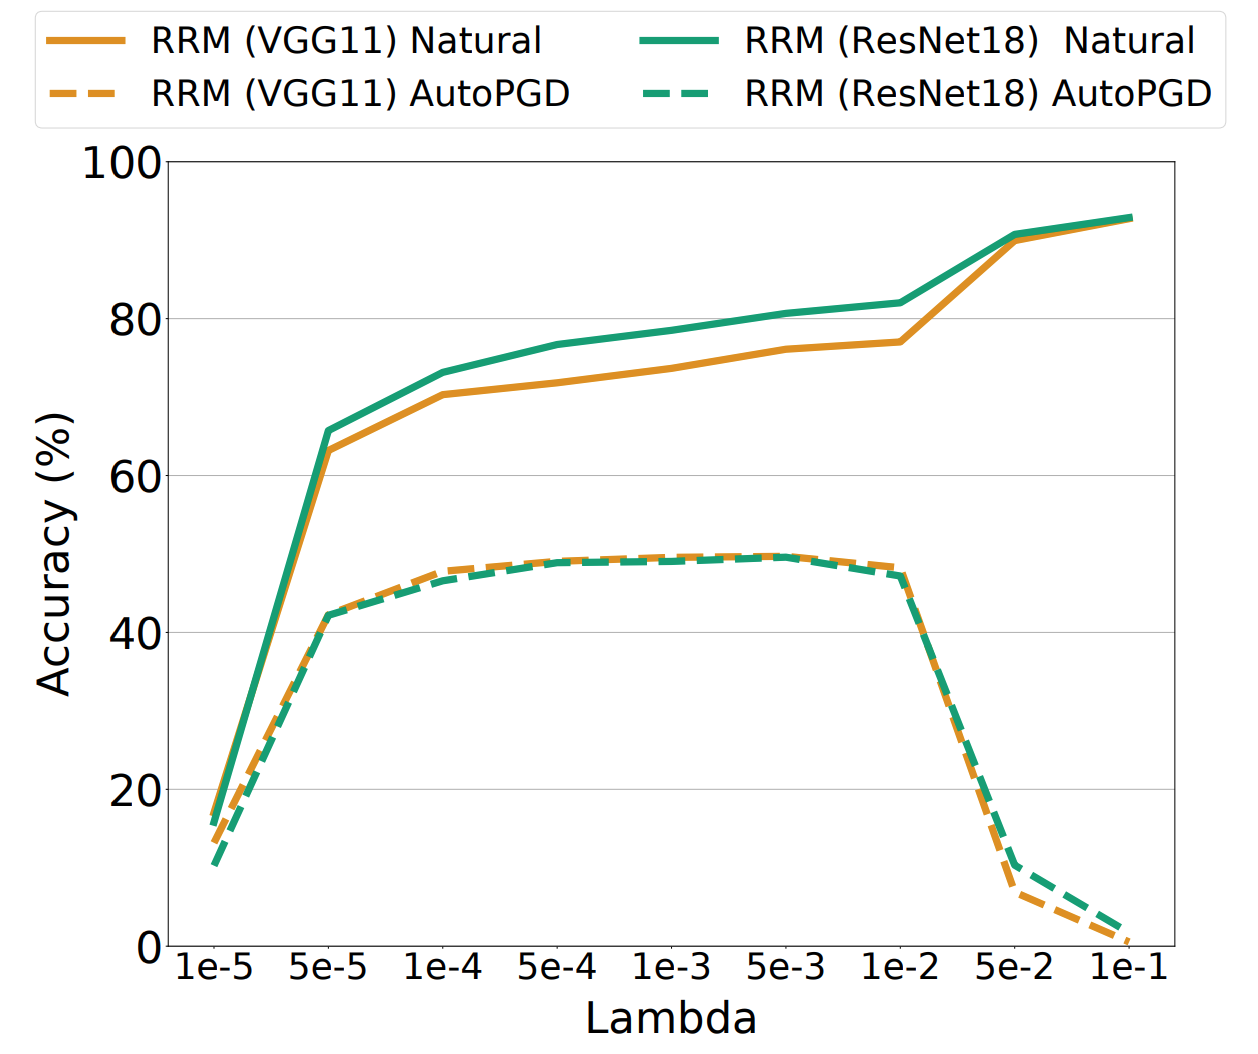
\includegraphics[scale=.3]{./images/tuning_lambda.png}
		%\caption{AutoPGD is the adversarial accuracy; VGG11 and ResNet18 are two different teachers for RRM students. In practice, $.005 < \lambda < .01$ worked best for this dataset}
		\caption{}
	\end{figure}
	
\end{frame}

%%%%%%%%%%%%%%%%%%%%%%%%%%%%%%%%%%%%%%%%%%%%%%%%%%
%%%%%%%%%%%%%%%%%%%%%%%%%%%%%%%%%%%%%%%%%%%%%%%%%%

\begin{frame}{Limit Testing}
	
	\begin{itemize}
		\item Hypothesize that training time per epoch roughly approximates a model's expressive power
		\item Found that simpler students struggle to learn from complex teachers because they are not complex enough to learn the robust features of the teacher
	\end{itemize}

	\begin{figure}
		\centering
		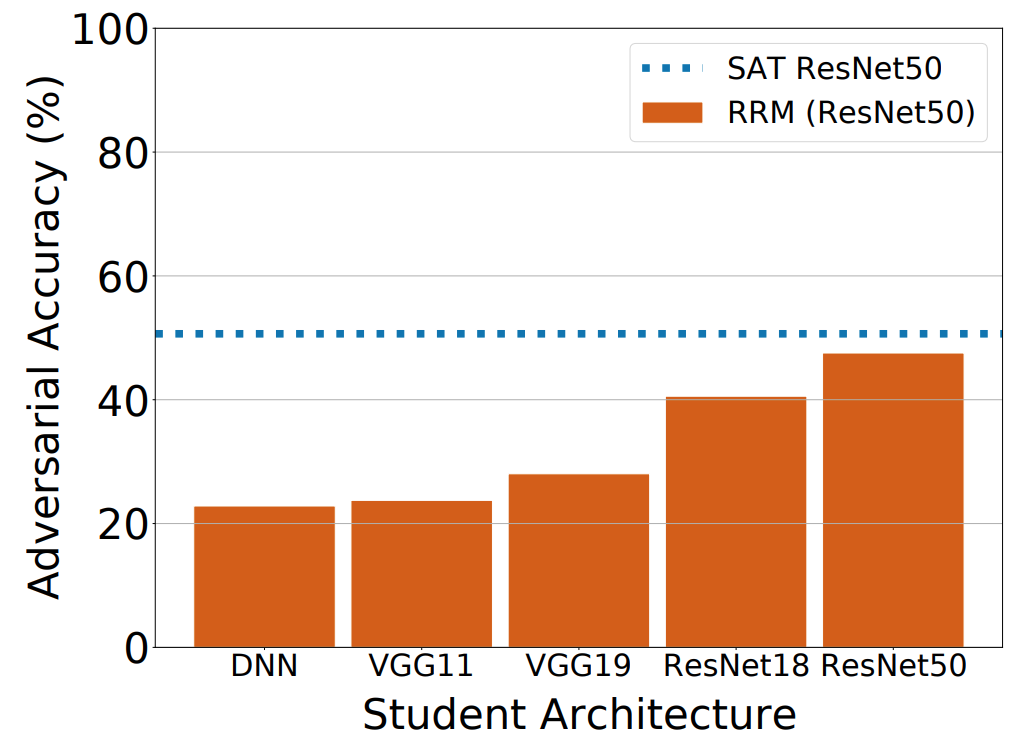
\includegraphics[scale=.40]{./images/limit_testing.png}
		\caption{}
	\end{figure}
	
\end{frame}

%%%%%%%%%%%%%%%%%%%%%%%%%%%%%%%%%%%%%%%%%%%%%%%%%%
%%%%%%%%%%%%%%%%%%%%%%%%%%%%%%%%%%%%%%%%%%%%%%%%%%

\begin{frame}{Limitations and Future Work}
	
	\begin{itemize}
		\item RRM still depends on a teacher model and the difficulties that go along with using AT to attain one
		\item This work only studies RRM with respect to DNNs and image classification
		\item AT is not the silver bullet for adversarial defense nor is it the only defense strategy
	\end{itemize}
	
\end{frame}

%%%%%%%%%%%%%%%%%%%%%%%%%%%%%%%%%%%%%%%%%%%%%%%%%%
%%%%%%%%%%%%%%%%%%%%%%%%%%%%%%%%%%%%%%%%%%%%%%%%%%

\begin{frame}{Conclusions}
	
	\begin{itemize}
		\item Introduced Robust Representation Matching (RRM) technique to transfer robustness between DNN models
		\item Demonstrated that RRM outperforms other adversarial training techniques and adversarial robustness transfer techniques
	\end{itemize}
	
\end{frame}

%%%%%%%%%%%%%%%%%%%%%%%%%%%%%%%%%%%%%%%%%%%%%%%%%%
%%%%%%%%%%%%%%%%%%%%%%%%%%%%%%%%%%%%%%%%%%%%%%%%%%

\begin{frame}{References}
	
	\bibliographystyle{./IEEEtran}
	\bibliography{presentation}
	
\end{frame}

\end{document}